\subsection[Thresholding]{Thresholding}

%\subsubsection[Training e test set]{Training e test set}


\begin{frame}
	
	\frametitle{Thresholding}
	
	La regressione logistica restituisce una probabilità.\\
	È possibile utilizzare la probabilità restituita ``così com'è'' (ad esempio, la probabilità che l'utente faccia clic su questo annuncio è 0,00023) o convertire la probabilità restituita in un valore binario (ad esempio, questa email è spam o non lo è).
	\begin{itemize}
		\item un modello di regressione logistica che restituisce \textbf{0,9995} per un particolare messaggio di posta elettronica prevede che è molto probabile che si tratti di \textbf{spam}
		\item al contrario, un altro messaggio di posta elettronica con un punteggio di previsione di \textbf{0,0003} sullo stesso modello di regressione logistica molto probabilmente \textbf{non è spam}
		\item tuttavia, che dire di un messaggio di posta elettronica con un punteggio di previsione di \textbf{0,6}?
	\end{itemize}
	
\end{frame}


\begin{frame}
	
	\frametitle{Thresholding: la soglia critica di classificazione}
	Per mappare un valore di regressione logistica a una categoria binaria, è necessario definire una \textbf{soglia di classificazione} (chiamata anche \textbf{soglia di decisione}).\\
	Un valore superiore a tale soglia indica ``spam''; un valore sotto indica ``non spam''.
	\newlinedouble
	Si è tentati di supporre che la soglia di classificazione debba sempre essere 0,5, ma le \textbf{soglie dipendono dal problema} e sono quindi valori che è necessario regolare.
	\newlinedouble
	Le sezioni seguenti \textbf{esaminano} più da vicino \textbf{le metriche} che è possibile utilizzare per valutare le previsioni di un modello di classificazione, nonché l'impatto della modifica della soglia di classificazione su queste previsioni.
	
\end{frame}


\subsubsection[Alcune metriche]{Alcune metriche}
\begin{frame}
	\frametitle{Thresholding: alcune metriche}
	
	\begin{scriptsize}
	
	\begin{columns}
		\column{0.5\linewidth}
		\begin{center}
			\begin{tabular}{cc|cc|c}
				& & \multicolumn{2}{c|}{$\widehat Y$}\\
				& & No & Sì & Total \\
				\hline
				\emph{Vera} & No & $n_{TN}$ & $n_{FP}$ & $n_{No}$ \\
				$Y$ & Sì & $n_{FN}$ & $n_{TP}$ & $n_{Si}$ \\
				\hline
				& Totale & $n_{\widehat No}$ & $n_{\widehat{Si}}$ & $n$
			\end{tabular}
		\end{center}
			
		\column{0.5\linewidth}
		\begin{figure}[!htbp]
			\centering
			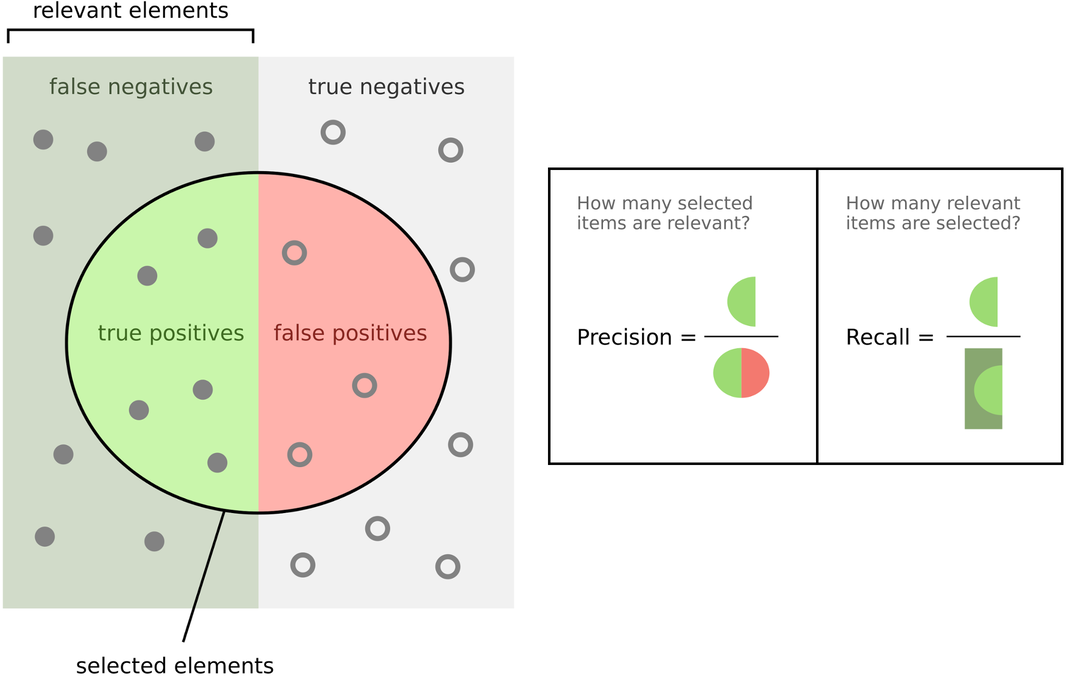
\includegraphics[width=0.8\linewidth]{images/supervised/z_algoritms_logistic_thresholding/PrecisionRecall.png}
%			\caption{}
		\end{figure}			
	\end{columns}

	
	\begin{itemize}
		\item \emph{Accuracy (o tasso d'errore totale)} = ${\displaystyle \frac{n_{FP}+n_{FN}}{n}}$: \% di osservazioni mal classificate
		\item \emph{FPR (tasso di falsi positivi)} = ${\displaystyle \frac{n_{FP}}{n_{No}}}$: \% di veri \rr{No}  classificati come \rr{Sì}
		\item \emph{FNR (tasso di falsi negativi)} = ${\displaystyle \frac{n_{FN}}{n_{Si}}}$: \% di veri \rr{Sì} classificati come \rr{No}
		\item \emph{Specificità} = ${\displaystyle \frac{n_{TN}}{n_{No}}}$ = 1 $-$ FPR: \% di veri \rr{No}  classificati come \rr{No}	
		\item \emph{Precision} = ${\displaystyle \frac{n_{TP}}{n_{\widehat{Si}}}}$: \% di predizioni \rr{Sì} classificate correttamente
		\item \emph{Recall (o sensitività, o TPR)} = ${\displaystyle \frac{n_{TP}}{n_{Si}}}$ = 1 $-$ FNR: \% di veri \rr{Sì} classificati \rr{Sì}
		\item Tutte queste misure variano con la soglia critica
	\end{itemize}
	
	\end{scriptsize}
\end{frame}


\begin{frame}
	\frametitle{Thresholding: alcune metriche al variare della soglia}
	
	\begin{center}
		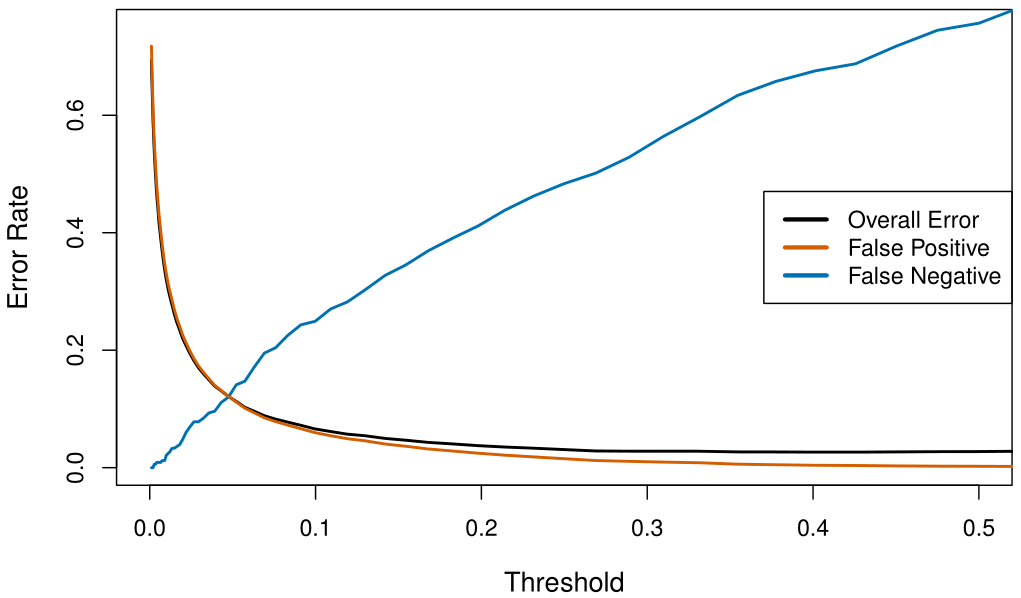
\includegraphics[scale=0.35]{images/supervised/z_algoritms_logistic_thresholding/thresholding_errors.png}
	\end{center}
	
	\begin{itemize}
		\item Per ridurre il TFN a un livello accettabile dobbiamo ridurre la soglia
	\end{itemize}
\end{frame}


\subsubsection[La scelta della soglia e l'accuracy paradox]{La scelta della soglia e l'accuracy paradox}
\begin{frame}
	\frametitle{Thresholding: la scelta della soglia e l'accuracy paradox}
	
	Al fine di di stabilire la soglia di classificazione ricordiamo il cosiddetto \textbf{accuracy paradox} secondo il quale:
	
	\begin{scriptsize}
	\begin{tcolorbox}[colback=yellow!10,colframe=blue!40!black!60]
	  The accuracy paradox for predictive analytics states that predictive models with a given level of accuracy may have greater predictive power than models with higher accuracy.\\
	  It may be better to avoid the accuracy metric in favor of other metrics such as precision and recall.
	\end{tcolorbox}
	\end{scriptsize}
	
	Questo è dovuto al fatto che i casi positivi e negativi spesso non sono equamente bilanciati all'interno dei campioni.\\
	Si potrebbe quindi scegliere di selezionare la soglia di classificazione attraverso l'utilizzo dell'\underline{\href{https://en.wikipedia.org/wiki/F1_score}{F1-Score}} ottenuto sul training-set al variare della soglia di classificazione.\\
	L'\textbf{F1-Score} è calcolato come una media armonica di precision e recall:
	$$F1 = \frac{2 * precision * recall}{precision + recall}$$
	
\end{frame}


\subsubsection[ROC]{ROC}
\begin{frame}
	\frametitle{Thresholding: la curva ROC e l'AUC}
	
	\begin{columns}
		\column{0.55\linewidth}
		\begin{itemize}
			\item Il \emph{grafico ROC} illustra:
			\begin{itemize}
				\item FPR sull'asse $x$		
				\item TPR sull'asse $y$
			\end{itemize}
			al variare della soglia critica
		
			\item L'\emph{Area Under the Curve, abbreviato in AUC} riassume il tradeoff fra i due tipi di errore.\\
				Quanto maggiore è l'AUC, tanto migliore risulta essere l'adattamento ai dati.
		\end{itemize}
			
		\column{0.45\linewidth}
		\begin{center}
			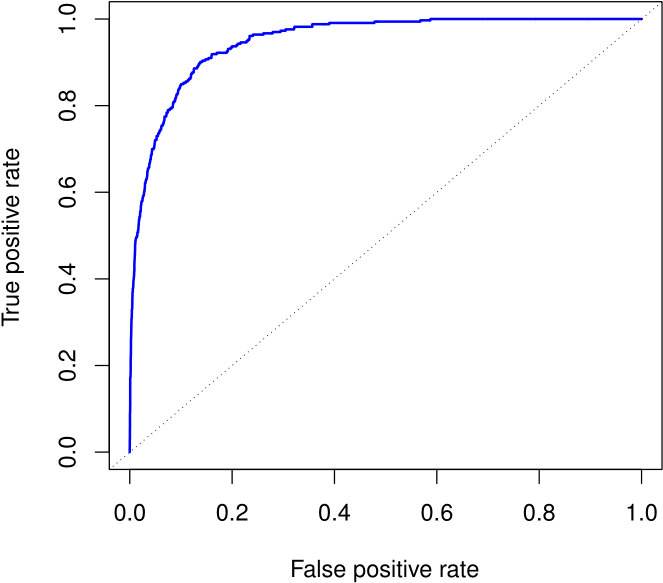
\includegraphics[width=1.0\linewidth]{images/supervised/z_algoritms_logistic_thresholding/roc.png}
		\end{center}			
	\end{columns}
	
\end{frame}


\subsubsection[AUC]{AUC}
\begin{frame}
	\frametitle{Thresholding: l'AUC}
	
	\begin{columns}
		\column{0.55\linewidth}
		L'AUC fornisce una misura aggregata delle prestazioni attraverso tutte le possibili soglie di classificazione.
		\newlinedouble
		L'AUC è desiderabile per i seguenti due motivi:
		\begin{itemize}
			\item l'AUC è invariante alla scala. Misura il grado di bontà delle previsioni, piuttosto che i loro valori assoluti.
			\item L'AUC è invariante alle soglie di classificazione. Misura la qualità delle previsioni del modello indipendentemente dalla soglia di classificazione scelta.
		\end{itemize}
			
		\column{0.45\linewidth}
		\begin{center}
			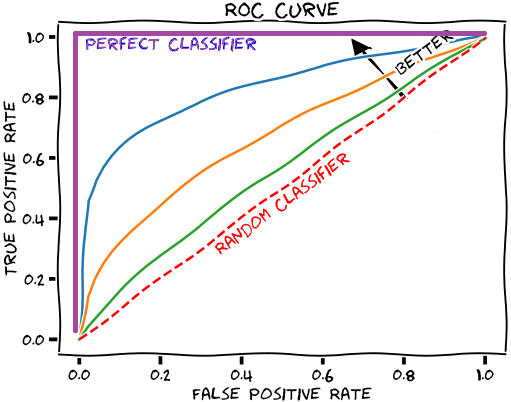
\includegraphics[width=1.0\linewidth]{images/supervised/z_algoritms_logistic_thresholding/roc-curve.png}
		\end{center}			
	\end{columns}
	
\end{frame}

